 \documentclass[a4paper,10pt]{article}
 \usepackage[utf8]{inputenc}  
 \usepackage[T1]{fontenc}
 \usepackage{graphicx}
 \graphicspath{{images/}} 
 
 \usepackage{wrapfig} 
 \usepackage{amsmath} 
 \usepackage{gensymb}
 \usepackage{fancyhdr}
 \usepackage{lastpage}
 \usepackage{textcomp}
 \usepackage{color}
 \usepackage{colortbl}
 \usepackage[table]{xcolor}
 \usepackage{courier}
 \usepackage{setspace}
 \usepackage{listings}
 \usepackage{ulem}%
 \usepackage{geometry}
 \usepackage{array}
 \geometry{a4paper,
 total = {140mm, 237mm},
 left = 35mm,
 top = 30mm}
 \newcommand{\minus}{\scalebox{0.6}[1.0]{$-$}} 
 \newcommand{\signature}[2]{%
  \par\nobreak\bigskip
  \begin{singlespace}%
  \mbox{}\hfill\begin{tabular}{p{8cm} }
      \rule{8cm}{0.5pt}\newline{}%
        \textbf{#1}\\%
       #2 %
  \end{tabular}%
  \end{singlespace}%
  \medskip%
 }
 \renewcommand{\lstlistingname}{Extrait de code}
 \lstset{
 language=Java,
 basicstyle=\scriptsize\ttfamily, 
 upquote=true,
 aboveskip={1.5\baselineskip},
 columns=fullflexible,
 showstringspaces=false,
 extendedchars=true,
 frame=single,
 breaklines=true,
 showtabs=false,
 showspaces=false,
 showstringspaces=false,
 identifierstyle=\ttfamily,
 keywordstyle=\color[rgb]{0.2,0.2,0.2},
 commentstyle=\color[rgb]{0.133,0.545,0.133},
 stringstyle=\color[rgb]{0.627,0.126,0.941},
 tabsize=5,
 }
 \pagestyle{fancy}
 \fancyhead[R]{Projet final SigmaPi}
 \fancyfoot[C]{\thepage}
 \fancyhead[L]{Loïc Gillioz, Loïc Fracheboud}
 \author{Loïc Gillioz, Loïc Fracheboud}
 \title{Informatique - Projet final \\ \Huge SigmaPi (Patapon-like)}
 \date{13 juin 2016}
 \begin{document}
 \maketitle

 \begin{figure}[!h]
 \centering
 \vspace{80pt}
 
\includegraphics[scale=0.2]{images/titre}
 \end{figure}
 \pagebreak
 
 \section{Description sommaire du jeu}
  SigmaPi est basé sur le jeu sorti sur PSP "Patapon". Ce dernier jeu, sorti en 2006, connu un grand succès et c'est désormais une des références des jeux de rythme. On y contrôle un groupe de guerriers par le biais de quatre tambours, en entrant des séquences (par exemple 3x carré puis 1x rond donne l'ordre d'avancer). On compte une petite dizaine de combinaisons, selon la version du jeu. Il est possible d'attaquer, de défendre, d'avancer, d'éviter, de charger une attaque, de faire pleuvoir, etc. Chacune de ces actions est exécutée à la suite d'une séquence spécifique. \\
Le but du jeu est donc de traverser des niveaux 2D à l'aide des différents ordres. Les niveaux du jeu original sont soit des niveaux de chasse (simples animaux pacifiques), de combat contre une tribu rivale, ou encore de combat contre un grand boss.
Dans notre jeu, nous n'avons implémenté que le type de niveau comprenant une tribu adverse.

 \paragraph{GitHub}
Afin de gérer au mieux les versions de notre code, nous avons utilisé les fonctions de GitHub. Vous pouvez donc retrouver tout l'historique de développement et tout le code à cette adresse : {\itshape https://github.com/loicfracheboud/SigmaPi}
  \begin{figure}[!h]
 \centering
 \vspace{5pt}
 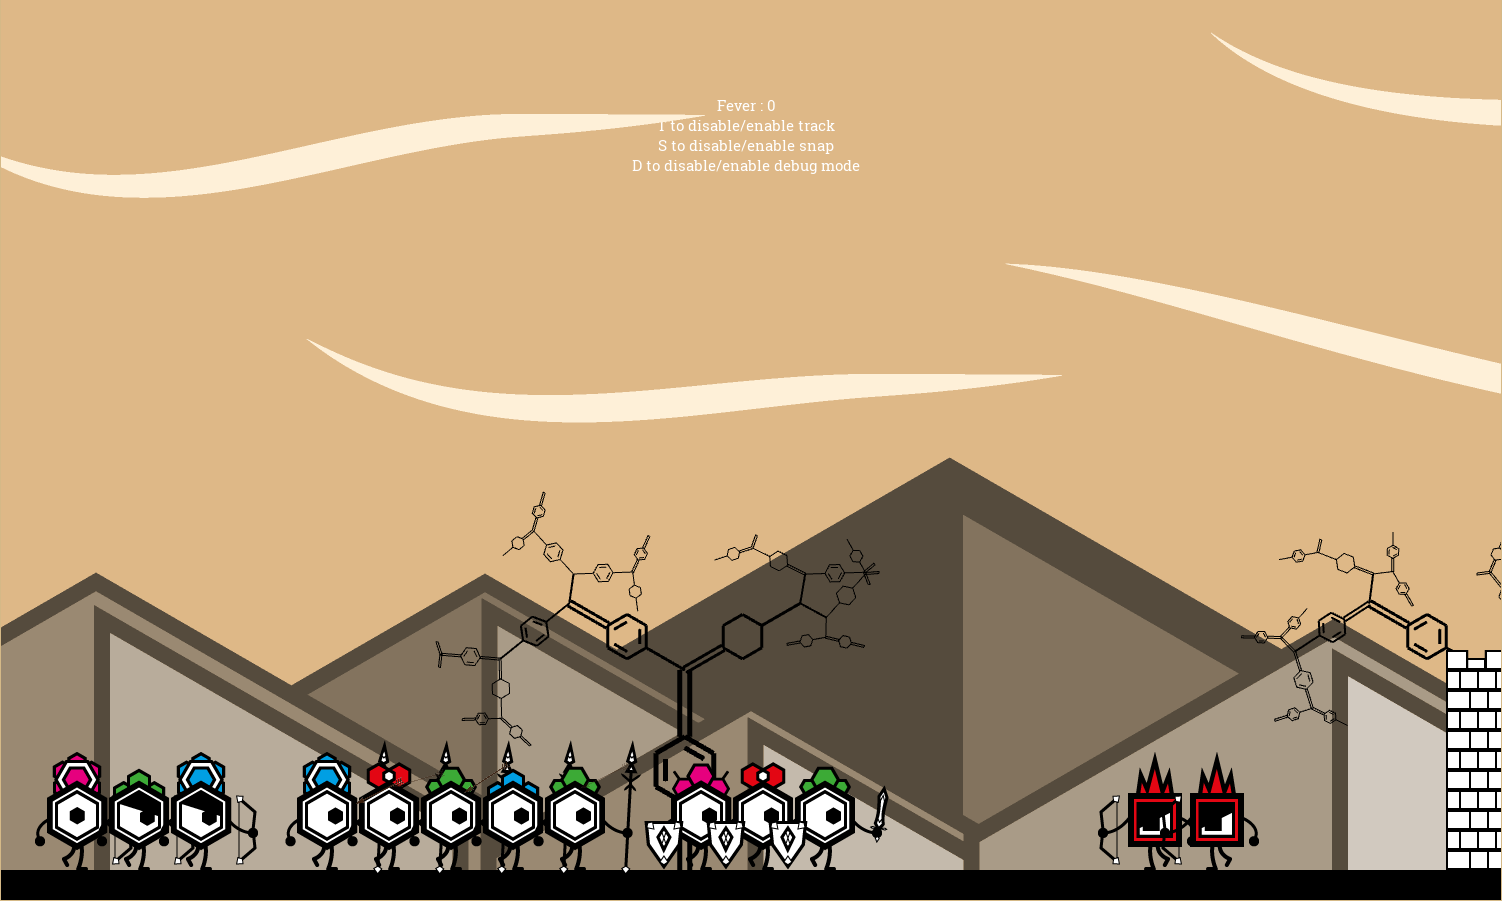
\includegraphics[scale=0.25]{images/menu}
 \caption{A gauche la compagnie du joueur et à droite deux archers ennemis}
 \end{figure}  
  \pagebreak
  
  \paragraph*{Structure UML}
  L'architecture du jeu comptant 46 classes, nous avons jugé utile de les séparer en plusieurs packages. On peut distinguer ci-dessous les packages dédiés à des tâches communes, graphismes, mécanique de jeux, etc.  
  
 \begin{figure}[!h]
 \centering
 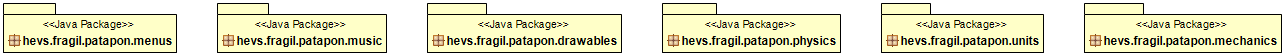
\includegraphics[scale=0.32]{images/Complete}
 \caption{Les 6 packages des classes}
 \end{figure}
  \paragraph{drawables}
  Ici nous avons toutes les classes qui s'occupent de la partie graphique du jeu, par exemple la classe SpriteSheet qui permet d'initialiser et travailler facilement avec les spritesheets. Pour les nuages et les montagnes, il est possible de donner un effet de parallaxe à l'aide d'un paramètre.
 \begin{figure}[!h]
 \centering
 \vspace{-45pt}
 
\includegraphics[scale=0.3]{images/legs}
 \end{figure}
  \begin{figure}[!h]
 \centering
 
\includegraphics[scale=0.3]{images/eyes}
 \caption{Spritesheet des jambes et des yeux des SigmaPi}
 \end{figure}
 Le dessin des SigmaPis est composé de 4 sprites superposés : les jambes, le corps, l'oeil, et les bras. Pour faciliter la tâche, les 4 différents sprites font la même taille de vignette et sont alignés selon le même offset, ce qui permet de les afficher tous à la même position, les uns après les autres.
 \begin{figure}[!h]
 \centering
 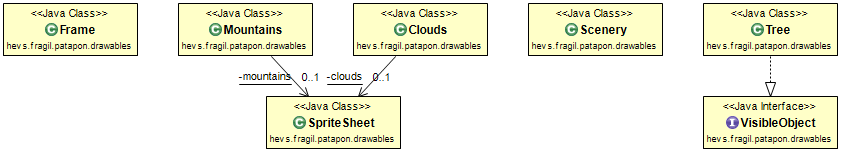
\includegraphics[scale=0.4]{images/Drawables}
 \caption{Structure sommaire du package drawables}
 \end{figure}
  \paragraph{mechanics}
  Ce package est axé sur la mécanique du jeu, c'est-à-dire toutes les classes qui permettent le fonctionnement des éléments de base, comme gérer l'état des unités, instancier les niveaux, gérer la compagnie du joueur.
 \begin{figure}[!h]
 \centering
 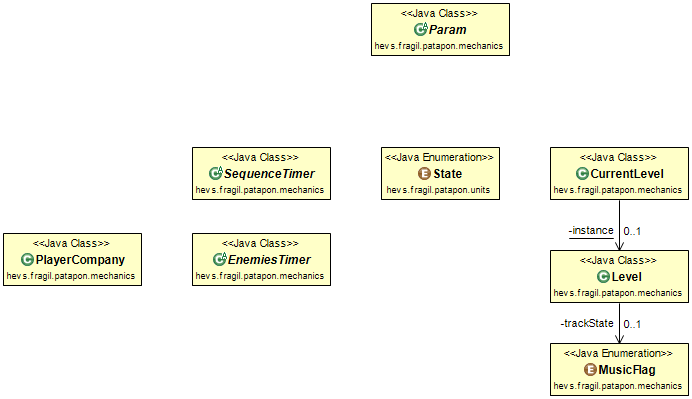
\includegraphics[scale=0.4]{images/Mechanics}
 \caption{Structure sommaire du package mechanics}
 \end{figure}
 
  \paragraph{menus}
  \begin{figure}[!h]
 \centering
 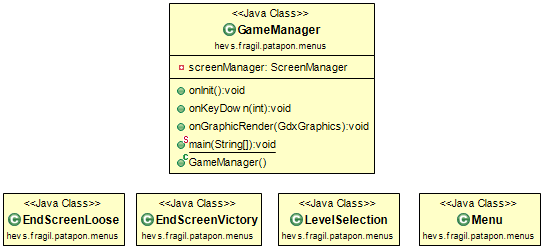
\includegraphics[scale=0.4]{images/Menus}
 \caption{Structure sommaire du package menus}
 \end{figure}
  Les différentes classes de ce niveau servent à générer des menus permettants de modifier les options du jeux, lancer une partie, etc. Pour l'instant nous n'avons pas implémenté ces fonctions, elles ne sont pas fondamentales et nous avons privilégié les autres fonctions.

  \paragraph{music}
  \begin{figure}[!h]
 \centering
 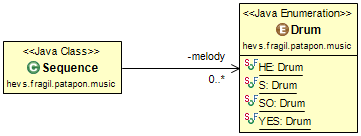
\includegraphics[scale=0.4]{images/Music}
 \caption{Structure sommaire du package music}
 \end{figure}
  Toute la gestion des séquences entrées par le joueur est traitée ici. On y crée les tambours, les séquences et on reconnait les séquence possibles tout en contrôlant le timing du joueur.
  
  \paragraph{physics}
  \begin{figure}[!h]
 \centering
 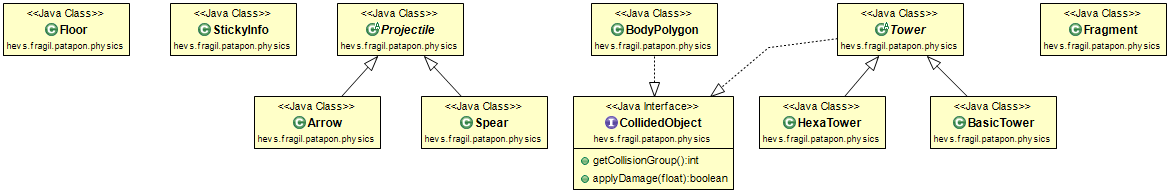
\includegraphics[scale=0.4]{images/Physics}
 \caption{Structure sommaire du package physics}
 \end{figure}
  La physique est utile à plusieurs fonctions du jeu, notamment pour les flèches/lances et les hitboxes des unités. Toutes les classes dans ce package influent sur la physique. Certaines sont également des objets affichables, mais nous avons préféré les mettre dans ce package plutôt que le package drawable, étant la place plus importante prise par la physique.
  \paragraph{units}
  \begin{figure}[!h]
 \centering
 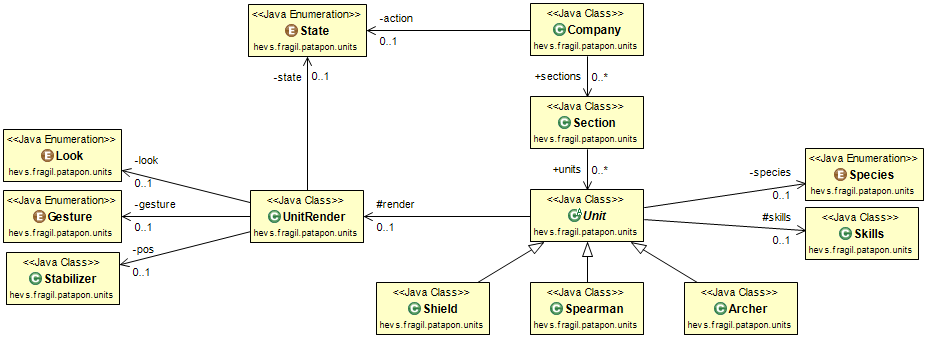
\includegraphics[scale=0.4]{images/Units}
 \caption{Structure sommaire du package units}
 \end{figure}
  Le package units contient toute la structure des compagnies, contenant sections, unités, etc. Quelques classes utiles pour les unités sont aussi présentes.
  
  \pagebreak 
  \section{Architecture}
  Eclaircissons quelques points intéréssants du fonctionnement du jeu.

  \paragraph{Intelligence artificielle (AI)}
  Dans le jeu il y a deux types d'AI. La plus évidente est celle des adversaires. Lors d'une partie, ils sont créés et placés à une position x dans le niveau. Lorsque le joueur s'en approchera suffisamment, ils vont devenir agressifs et attaquer. Sachant que chaque unité à une certaine portée, ils vont se déplacer dans une zone définie afin de pouvoir nous atteindre.
  \newline Pour le joueur il existe un système similaire. C'est-à-dire que ses unités possèdent aussi une zone dans laquelle elle peuvent se déplacer pour faire correspondre leur portée à la position de la victime. La différence par rapport aux unités ennemies est que leur zone d'action bouge en fonction des actions du joueur.
  \newline Le deuxième point intéressant qui ne concerne que le joueur, c'est la faculté des unités à se regrouper selon un ordre bien défini lors des déplacements.
  \newline Tout ceci est possible grâce à une série de calculs déterminant les déplacements potentiels et leurs conséquences. En fonction de cela (et de la volonté du joueur), le système donne les instructions finales. Le code est entièrement commenté pour un bonne compréhension des différentes étapes de décision des unités.
   
    \paragraph{Vol des projectiles}
  Les projectiles sont respectivement les flèches ou les lances. Dans les 2 cas, leur trajectoire en vol est gérée par la physique selon le modèle dans le vide. La simulation dans le vide pose problème car les projectiles n'ont aucune raison de voler comme dans la vraie vie. En effet, l'empennage des flèches et leur centre de gravité dévié les fait voler en tournant pour se planter dans le sol ou les ennemis. Sans cela, les flèches ne tournent pas et ce n'est vraiment pas réaliste.\\
  Pour créer une trajectoire réaliste, on applique un moment sur le projectile proportionnel à l'angle qu'il forme avec le sol. Cette technique a été inspirée du tutoriel d'iForce2D\footnote{Sticky Projectiles, http://www.iforce2d.net/b2dtut/sticky-projectiles}, qui parlait de créer des flèches qui se plantent à l'impact. \\
  Pour les faire se planter à l'impact, là aussi nous nous sommes largement inspirés du tutoriel qui proposait de créer des joints en passant des "StickyInfo", ce que nous avons entièrement repris. \\ 
  Lors de la collision, on applique les dégâts du projectile à la box de la victime. Ensuite, on change le CollisionGroup du projectile pour éviter d'autres collisions avec les autres victimes aux alentours, notamment lors de la mort de la victime (celle-ci bascule sur le côté).
 \pagebreak 
  \paragraph{Tours et explosions}
  Les tours à détruire sont premièrement composées d'un box physique statique, qui empêche n'importe quel autre objet de la déplacer. Cela évite des problèmes de collisions et de forces inutiles. Lors de réception des dégâts, la tour baisse ses points de vie. Lorsque la tour n'a plus de points de vie, on détruit sa hitbox statique et on la remplace par une série de fragments, auxquels on applique directement une force pour la faire exploser. Cette force est aléatoire. Pour éviter des collisions hasardeuses avec la compagnie du joueur, les fragments sont dans le même CollisionGroup que les unités alliées.
 \begin{figure}[!h]
 \centering
 \vspace{-10pt}
 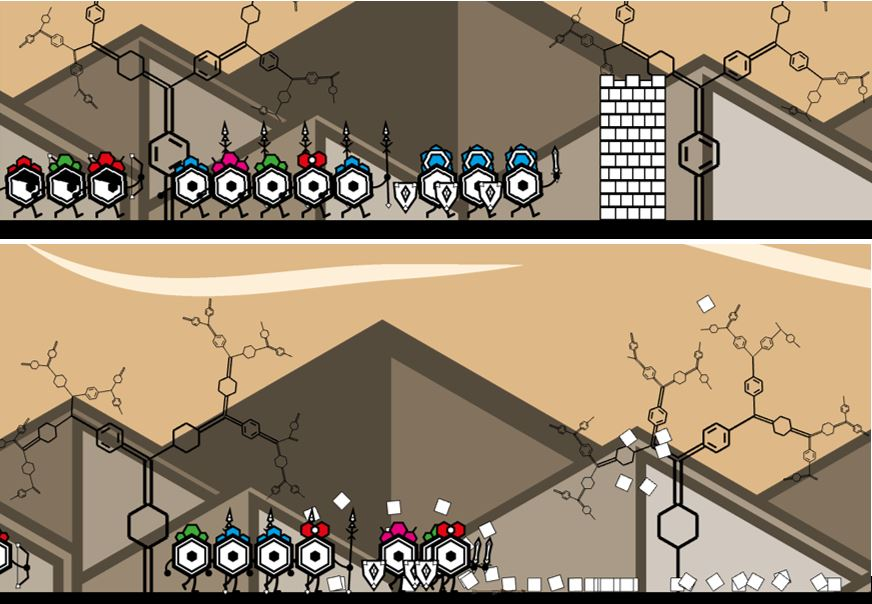
\includegraphics[scale=0.45]{images/towers}
 \caption{La tour avant et après}
 \end{figure}

  
  \paragraph{Arbres récursifs}
  Dans le jeu on peut voir des arbres qui ondulent selon un vent fictif. Ces arbres sont générés avec les principes de récursivité et un peu d'aléatoire. Nous avons défini quelques motifs de base (ligne simple/double, hexagone vide/rempli, etc) et quelques règles (chaque section est composée d'un élément ligne, puis un élément hexagone et à nouveau une ligne ou juste un élément ligne seul). A partir de là on peut générer un arbre. 
Dans la classe de gestion du décor on peut donc appeler cette fonction de dessin d'arbre pour en faire une forêt. Dans notre cas, une forêt représente l'ensemble des arbres présents sur le niveau. La génération d'une forêt prend quelques paramètres en entrée et génère ensuite le nombre d'arbre désirés, avec une taille et un niveau de récursivité moyens afin d'avoir un résultat cohérents visuellement.
  \newline Reprenons l'arbre de la section précédente et comparons le à son voisin. On voit qu'ils ont le même niveau de récurivité, mais pas la même taille, ni la même structure.
 \begin{figure}[!h]
 \centering
 \vspace{-10pt}
 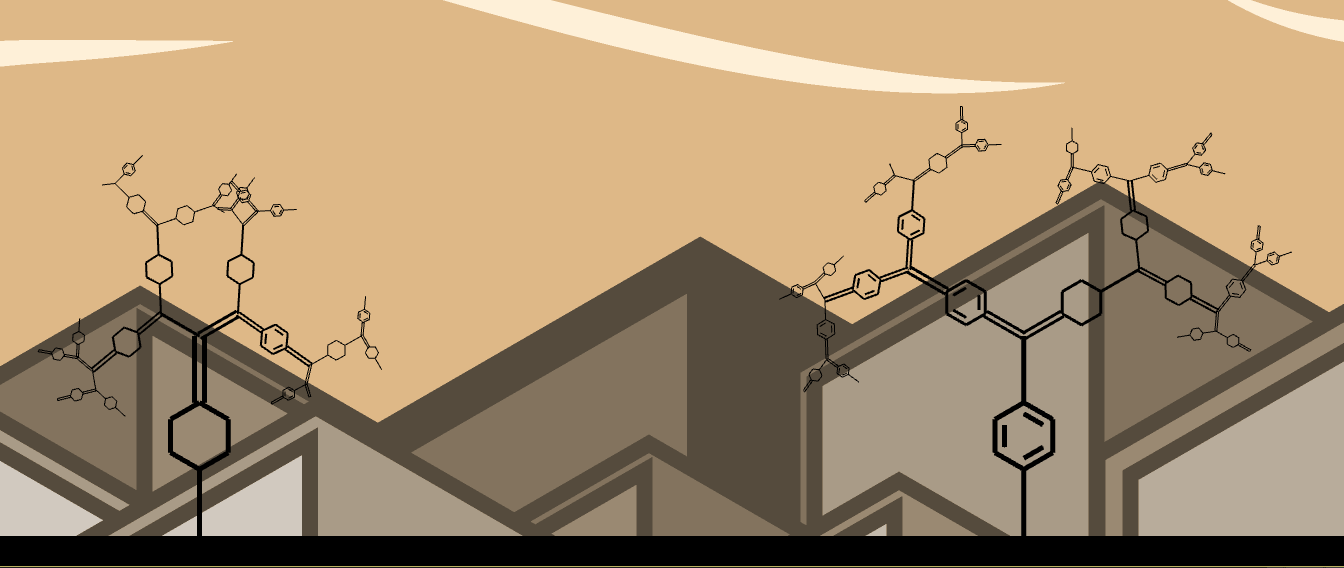
\includegraphics[scale=0.22]{images/trees}
 \caption{Deux arbres générés par le jeu}
 \end{figure}
  
  \pagebreak 
  \section{Confrontation au planning}
  Maintenant que le projet est terminé, nous pouvons tirer un bilan sur le planning prévu et celui réalisé. Pour rappel, nous avions planifié le travail comme suit :
  \paragraph{}
 \newcolumntype{M}[1]{>{\raggedright}m{#1}}
 {\rowcolors{1}{lightgray}{white}
\begin{tabular}{M{9cm}lc}
\bf Fonctionnalité & \bf  Date & \bf Importance \tabularnewline
Gestion des séquences de notes & Implémenté & +++ \tabularnewline
Gestion des actions par fonction (p.ex. les archers tirent des flèches, lanciers des lances, les épéistes frappent mais ne lancent rien) & 06.05.2016 & +++ \tabularnewline
    Déplacement de la caméra selon la position des SigmaPis & 12.05.2016  & +++\tabularnewline
    Utilisation de la physique pour les objets balistiques et des collisions & 20.05.2016 & ++ \tabularnewline
    Utilisation des collisions pour appliquer les dégâts aux unités & 20.05.2016 & ++\tabularnewline
    Adaptation des aptitudes des SigmaPis selon leur niveau et race & 12.06.2016 & ++\tabularnewline
    Création d'animations sans SpriteSheets (transformations par calcul) & 12.06.2016 & + \tabularnewline
Décors récursifs & 26.05.2016 & + \tabularnewline
    Mise en place d'un scénario & 12.06.2016 & -- \tabularnewline 
    Réserve pour les imprévus & 19.06.2016 & *left blank* \tabularnewline
\end{tabular}}

 \paragraph{}
 Nous n'avons pas réellement respecté le planning, en fait des éléments se sont retrouvés très vite codés dans la timeline (par exemple les arbres récursifs ou les animations sans SpriteSheets) tandis que d'autres ne sont pas encore implémentés, notamment les différents niveaux des SigmaPis, l'équilibrage, etc.
 \newline Nous avons plutôt concentré nos efforts sur une architecture de jeux puissante par sa souplesse. De cette façon, le gameplay sera relativement simple à implémenter puisqu'il n'y aura pas à créer beaucoup de choses, il suffira grossièrement d'instancier les éléments nécessaires à un jeux agréable (niveaux de puissance des unités, modification de leurs paramètres, génération de décors uniques, etc..).
 
 \pagebreak
 \section{Conclusion}
 Le jeu est loin d'être fini du point de vue du gameplay, il manque en effet beaucoup d'éléments pour se rapprocher de la richesse de Patapon. En revanche nous avons maintenant une base solide qui offre l'architecture nécessaire au jeu.
 \newline Ce projet nous a beaucoup plu par tous les aspects abordés, que ce soit l'application de principes vus rapidement en théorie (ou pas du tout !), l'utilisation de GitHub, de fonctions Java inconnues ou encore des merveilles d'Illustrator pour générer les spritesheets. Créer ce jeu a été un réel investissement personnel et l'on ne compte plus les soirées passées avec le sourire (parfois un peu moins souriant, mais quand même !).
En résumé, beaucoup de plaisir !
Merci à vous pour votre investissement, votre intérêt et votre constante et contagieuse bonne humeur !

 \vspace{30pt}
 \begin{wrapfigure}[0]{r}{6cm}
 \vspace{-52pt}
 \centering
 
\includegraphics[scale=0.5]{signgillioz}
 \end{wrapfigure}
 \signature{Loïc Gillioz}{Sion, le 19 juin 2016} 
 
 \begin{wrapfigure}[0]{r}{6cm}
 \vspace{-52pt}
 \centering
 
\includegraphics[scale=1]{signfracheboud}
 \end{wrapfigure}
 \signature{Loïc Fracheboud}{Sion, le 19 juin 2016} 
 
  \begin{figure}[!h]
 \centering
 \vspace{100pt}
 
\includegraphics[scale=0.3]{images/Broken-Games}
 \end{figure}
 
 \end{document}